%%%%%%%%%%%%%%%%%%%
%% KAPITEL Intro %%
%%%%%%%%%%%%%%%%%%%
\section{Einführung}
% JONAS
% was ist es, wer benutzt es, wofür braucht man es
% erreichbar durch Transaktion SWDD, im SAP System eingebaut usw

\subsection{Funktionen des Builders}
\label{sec:builder-funktionen}
% MARCO
% welche Funktionalitäten hat der Builder...
Im Folgenden sollen nun zuerst die wichtigsten Funktionen des \gls{sap} Workflow Builders erklärt werden. Danach folgt im Kapitel \nameref{sec:builder-elemente} eine breiter gefächerte tabellarische Übersicht. Dort sind auch die Symbole der Schrittypen mit aufgeführt. 

Beim ersten Start des Programms wird dem Benutzer statt einer leeren Arbeitsfläche der minimale Aufbau eines Workflows im \gls{sap}-System angezeigt. Dieser besteht aus dem Startereignis "Workflow gestartet" und dem Endereignis "Workflow beendet". Dazwischen können beliebige Schritte an Stelle des unbekannten Schrittes (gekennzeichnet durch einen Pfeil auf weißem Hintergrund) eingefügt werden.

\begin{figure}[H]
	\begin{center}
	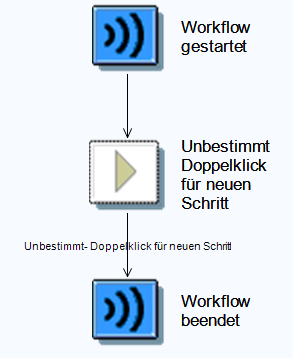
\includegraphics[width=150px]{grafiken/wf-builder_new-wf.png}
	\caption{Der initiale Workflow des Builders}
	\vspace{-10pt}
	\label{abb:SAPHanaAbout}
	\end{center}
\end{figure}

\subsubsection*{Aktivität}
Der wichtigste Schritttyp ist die Aktivität, welche verschiedene Aufgaben erfüllen kann. Der Benutzer kann entweder einen \gls{abap} \gls{objekttyp} und eine zugehörige Methode oder eine im System vorhandene und schon definierte Aufgabe auswählen. Die entsprechende Aktivität wird dann vom System automatisch gestartet, wenn die Stelle im laufenden Workflow erreicht wird.

\subsubsection*{Web-Aktivität}
Mit Hilfe dieses Schrittes wird aus dem internen Workflow heraus ein XML-Dokument an eine URL gesendet. Der Empfänger kann beispielsweise ein anderes System sein, welches daraufhin einen eigenen Workflow startet. Alle \gls{sap}-Systeme stellen einen Service zur Verfügung, welcher in diesem Fall automatisch einen weiteren Workflow starten kann.

\subsubsection*{Mail versenden}
Dieser Schritt versendet eine Nachricht innerhalb des \gls{sap}-Systems. Der Empfänger (es sind mehrere Empfänger möglich) kann diese im internen Postfach abrufen. Der Text der Mail wird bei der Definition des Schrittes festgelegt, wobei Variablen verwendet werden können, welche zur Laufzeit mit den entsprechenden Werten gefüllt werden.

\subsubsection*{Formular}
Ein Formular kann innerhalb des Workflows zur Anzeige von Daten oder deren Bearbeitung durch den Endnutzer verwendet werden. Nachdem bei der Definition des Schrittes die zu bearbeitenden Daten angegeben wurden, erzeugt das Workflow-System automatisch das zugehörige Formular, welches noch bearbeitet werden kann. 

\subsubsection*{Benutzerentscheidung}
Eine Benutzerentscheidung kann mit einem Text versehen werden, welcher dem Endnutzer erklärt, welche Entscheidung er treffen muss. Der Workflow kann so konfiguriert werden, dass er, je nachdem welche der vorgegebenen Antwortmöglichkeiten ausgewählt wurde, einen anderen Pfad wählt.

\subsubsection*{Bedingungen}
Die Schritte Bedingung und Mehrfachbedingung bestimmen, ähnlich der Benutzerentscheidung, den weiteren Ablauf des Workflows. Der Unterschied besteht darin, dass das System die Entscheidung eigenständig nach vorgegebenen Bedingungen fällt und der Benutzer keinen Einfluss darauf hat.

\subsubsection*{Schleifen}
Die WHILE- und UNTIL-Schleifen können eingesetzt werden, wenn ein bestimmter Teil des Workflows ausgeführt werden soll, während eine bestimmte Bedingung wahr ist oder so lange, bis sie eintritt. Schleifen können sämtliche Schrittypen (auch weitere Schleifen) enthalten und sorgen dafür, dass ein Workflow übersichtlich bleibt. 

\cite{SAPHelp}

\subsection{Builder Elemente}
\label{sec:builder-elemente}
% MARCO, STEFFEN
% tabelle mit elementen..
% was ist wofür gedacht

%%%%%%%%%%%%%%%%%%%%%
%% KAPITEL HandsOn %%
%%%%%%%%%%%%%%%%%%%%%
%% MARCO
%%%%%%%%%%%%%%%%%%%%%
\section{Hands On}

\subsection{Erster Beispielworkflow}
\label{sec:builder-1-bsp}
% kleiner sinnloser workflow (schleife,...)

\subsection{Zweiter Beispielworkflow}
\label{sec:builder-2-bsp}
%

\subsubsection{Vorstellung des Workflows}
\label{sec:builder-2-bsp-vorstellung}
% wofür ist der workflow gut, was soll er tun (aus anwendersicht)

\subsubsection{Umsetzung des Workflows}
\label{sec:builder-2-bsp-umsetzung}
% technische sicht, "`klickbares"' howto

%%%%%%%%%%%%%%%%%%%%%%%%%%
%% KAPITEL Fremdsysteme %%
%%%%%%%%%%%%%%%%%%%%%%%%%%
%% JONAS 
%%%%%%%%%%%%%%%%%%%%%%%%%%
\section{Schnittstellen}
%http://scn.sap.com/docs/DOC-31056
%Many SAP applications deliver workflows as content with the %SAP application. ERP, CRM, SRM are examples of SAP %applications that provide ready-to-use workflows. You can %change these workflows to reflect your company processes by %using the graphical workflow builder or build your own from %scratch.

\subsection{XML}
\label{sec:export-xml}
% was ist dieses Format
% in welche Programme kann man es importieren?

\gls{xml} ist die Abkürzung für E\textbf{x}tensible \textbf{M}arkup \textbf{L}anguage und bezeichnet eine Auszeichnungssprache. Durch diese können hierarchisch strukturierte Daten in Textform dargestellt werden. \gls{xml} besteht aus Elementen, deren Name relativ frei gewählt werden darf. Elemente haben einen Anfangs- (<elementName>) und einen Endtag (</elementName>) und zwischen diesen können wiederum weitere Elemente, Text oder andere Knoten enthalten sein. 

Das WorldWideWebConsortium, kurz W3C, hat \gls{xml} als eine Metasprache definiert, auf deren Basis anwendungsspezifische Auszeichnungssprachen entwickelt werden können. Diese werden beschrieben durch ein Schema, welches festlegt, welche Elemente verwendet werden dürfen und welches Verhalten diese aufweisen.

\subsection{BPML}
\label{sec:export-bpml}
% was ist dieses Format
% in welche Programme kann man es importieren?

Die \textbf{B}usiness \textbf{P}rocess \textbf{M}odeling \textbf{L}anguage (\gls{bpml}) ist genau wie XHTML auch eine Ableitung von \gls{xml}.

\subsection{SAP Fremdsysteme}
\label{sec:export-sap}
